\documentclass[addpoints,11pt,a4paper]{exam}
\usepackage{anysize}
\marginsize{1cm}{2cm}{.5cm}{1cm}
\usepackage[utf8]{inputenc}
\usepackage[magyar]{babel}
\usepackage{t1enc}
\usepackage{nicefrac}
\usepackage{siunitx}
\usepackage{multicol}
\usepackage{mailmerge}
\usepackage{amsmath}
\usepackage{amssymb,wasysym}
\usepackage{dsfont}
\pagestyle{empty}
\pointname{ pont}
\usepackage{multicol}

\usepackage{tikz}
\usetikzlibrary{patterns}
\begin{document}
	
	
	\begin{questions}
		\question A fémezüstből megvilágítás hatására kilépő elektron kilépési munkája $0,69 \mathrm{~aJ}$.  
		\begin{parts}
			\part Legalább mekkora legyen annak a fénynek a frekvenciája, amelynek hatására az elektron kiléphet az ezüst felületéről?
			\part Milyen fényről lehet szó: infravörös, látható vagy ultraibolya fényről?
		\end{parts}
		
		\question Vizsgáljunk egy $0,02\mathrm{~W}$ teljesítményű, $630\cdot 10^{-9}\mathrm{~m}$ hullámhosszon sugárzó héliumneon lézert!
		\begin{parts}
			\part Határozza meg a lézer által kibocsátott fény egy fotonjának energiáját!
			\part Határozza meg a fényforrás által két másodperc alatt kibocsátott fotonok számát! 
		\end{parts}
		
		\question A hidrogénatom energiaszintjeit az  $E_n=-\dfrac{2,2}{n^{2}}\mathrm{~aJ}$ összefüggéssel írhatjuk le. (Ahol n= 1,2,3,… pozitív egész szám, amely a különböző energiaszinteket jelöli.) Mekkora annak az elektromágneses hullámnak a hullámhossza, amelyet a hidrogén akkor sugároz ki, amikor egy elektronja a 2. energiaszintről a legmélyebb energiaszintre ugrik?
		
		\question Tegyük fel, hogy egy hidrogénatom fotont bocsát ki, miközben elektronja az $n = 5$ főkvantumszámmal jelzett állapotból az $n = 3$ főkvantumszámmal jelzett állapotba jut. Az így kibocsátott fotont elnyeli egy másik hidrogénatom, amely így ionizálódik. Hányas főkvantumszámú állapotban lehetett az ionizált hidrogénatom elektronja a foton elnyelése előtt? A hidrogénatom elektronjának energiája az $n$ főkvantumszámmal jelzett állapotban $E_n = -\dfrac{13,6}{n^{2}}\mathrm{~eV}$. 
		
		\question Egy $10\mathrm{~W} $ teljesítményű fényforrás $450\mathrm{~nm}$ hullámhosszúságú kék fényt bocsát ki.
		\begin{parts}
			\part Mekkora egy foton energiája?
			\part Hány foton hagyja el a fényforrást 1 perc alatt? 
		\end{parts}
		 
		 \question A fényelektromos jelenség során fotonok elektronokat löknek ki egy ezüstlemezből. Az alábbi táblázat a becsapódó fotonok energiáját és a kilépő elektronok mozgási energiáját tartalmazza. (Ez utóbbit feszültségmérés segítségével határozták meg.) A táblázatból egy adat hiányzik.
		 \begin{center}
		 	$\begin{array}{|c|c|c|c|c|c|c|}
		 	\hline \text { foton energiája - }(\mathrm{eV}) & 5,12 & 5,88 & & 6,92 & 7,55 & 7,92 \\
		 	\hline \text { elektron energiája - }(\mathrm{eV}) & 0,41 & 1,12 & 1,52 & 2,17 & 2,77 & 3,20 \\
		 	\hline
		 \end{array}$
		 \end{center}
		 \begin{parts}
		 	\part Ábrázolja grafikusan a kilépő elektronok energiáját a fotonok energiájának függvényében!  
		 	\part A fenti adatok segítségével határozza meg, hogy mennyi a kilépési munka az ezüst esetében!  
		 	\part Legfeljebb mekkora lehet a fotonok hullámhossza, hogy az elektronkilökés lejátszódjon?  
		 	\part Számítással vagy a grafikon alapján adja meg a táblázatból hiányzó adatot! 
		 \end{parts}
		 \begin{center}
		 	\includegraphics[width=\textwidth]{abra01}
		 \end{center}
	\begin{center}
			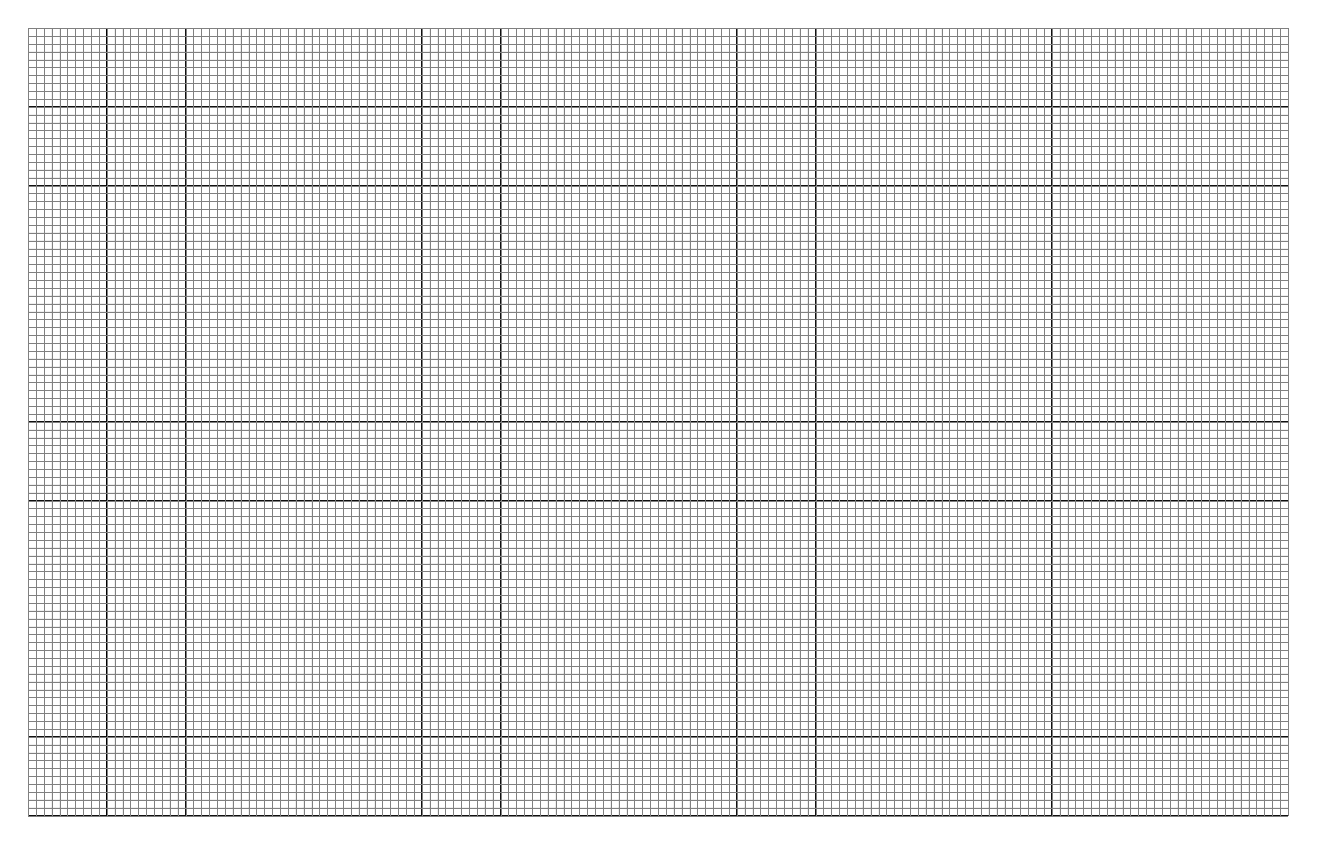
\begin{tikzpicture}[x=1mm, y=1mm, dotted/.style={pattern=dots}]
			
			\draw[step=10mm, line width=0.15mm, dotted] (0,0) grid (160mm,100mm);
			\draw[step=1mm, line width=0.035mm, dotted, gray] (0,0) grid (160mm,100mm);
		\end{tikzpicture}
	\end{center}
		  
		  \question Az elektronmikroszkóppal számottevően jobb felbontást lehet elérni, mint a
		  hagyományos mikroszkóppal, azaz lényegesebben apróbb tárgyakat is meg lehet
		  vizsgálni vele. Vajon miért?
		  \begin{choices}
		  	\choice Mert az elektronok sokkal kisebbek, mint a fotonok.
		  	\choice Mert az elektronnyaláb elektronjainak de Broglie-hullámhossza sokkal kisebb
		  	lehet, mint a látható fény fotonjainak hullámhossza.
		  	\choice Mert a felhasznált elektronok mozgási energiája kisebb, mint a látható fény
		  	fotonjaié.
		  
		  \end{choices}
		 
		 \question Egy elektront U feszültségű homogén elektromos térben gyorsítottunk. Hogyan
		 változott eközben a de Broglie-féle hullámhossza?
		 \begin{choices}
		 	\choice Nőtt.
		 	\choice Csökkent.
		 	\choice Nem változott.
		 \end{choices}
		 
		 \question Egy elektronmikroszkóp segítségével különböző tárgyakról készítettünk képeket.
		 Melyik kép készítésénél volt az elektronnyaláb gyorsító feszültsége a legnagyobb?
		 \begin{center}
		 	\includegraphics[width=\textwidth]{abra02}
		 \end{center}
		\begin{choices}
			\choice Az első felvétel készítésénél.
			\choice A második felvétel készítésénél.
			\choice A harmadik felvétel készítésénél.
			
		\end{choices}		  
		
		\question Mitől függ egy atom de Broglie hullámhossza?
		\begin{choices}
			\choice Az atom fajtájától – minden atomnak jellegzetes de Broglie hullámhosszai vannak,
			ami az emissziós színképében kimutatható.
			\choice A lendületétől – az atom de Broglie hullámhossza csökken ha az atom sebessége
			vagy tömege növekszik.
			\choice A tömegétől – minél nehezebb egy atom, annál nagyobb a de Broglie
			hullámhossza.
		\end{choices}
		
		\question Két (a fénysebességnél sokkal lassabban mozgó) részecske tömege $m_1$ és $m_2$.
		Mozgási energiájuk megegyezik. Mekkora a de Broglie-hullámhosszuk aránya?\\
		\begin{oneparchoices}
			\choice $\dfrac{\lambda_{1}}{\lambda_{2}} = \dfrac{m_{1}}{m_{2}}$ 
			\choice $\dfrac{\lambda_{1}}{\lambda_{2}} = \dfrac{m_{2}}{m_{1}}$ 
			\choice $\dfrac{\lambda_{1}}{\lambda_{2}} = \sqrt{\dfrac{m_{1}}{m_{2}}}$ 
			\choice $\dfrac{\lambda_{1}}{\lambda_{2}} = \sqrt{\dfrac{m_{2}}{m_{1}}}$ 
		\end{oneparchoices}
		
		\question Az elektronok hullámtulajdonságát kísérletileg csak jóval de Broglie
		hipotézisének felállítása után bizonyították. A kísérlet lényegére vonatkozó alábbi
		megállapítások közül melyik a helyes?
		\begin{choices}
			\choice A kísérletben polarizált elektronnyalábot sikerült létrehozni, ezzel bizonyítva a
			hullámtulajdonságot.
			\choice A kísérletben az elektron-interferenciát sikerült létrehozni két résen, ezzel
			bizonyítva a hullámtulajdonságot.
			\choice A kísérletben a fotoeffektus fordítottját sikerült létrehozni, ezzel bizonyítva az
			elektron hullámtulajdonságát.
		\end{choices}
		
		\question Hogyan lehet egy elektron de Broglie-hullámhosszát növelni?
		\begin{choices}
			\choice  Úgy, hogy növeljük az elektron sebességének nagyságát.
			\choice Úgy, hogy csökkentjük az elektron sebességének nagyságát.
			\choice Úgy, hogy megváltoztatjuk a haladásának irányát mágneses térrel.
			\choice Sehogyan, az elektron de Broglie-hullámhossza adott konstans.
		\end{choices}
		
		\question Melyik részecskének nagyobb a de Broglie-hullámhossza: az elektronnak vagy
		pedig a protonnak?
		\begin{choices}
			\choice Az elektronnak, mivel az sokkal könnyebb, így gyorsabban is mozog, mint a
			proton.
			\choice A protonnak, mivel a hullámhossz a tömeggel arányos.
			\choice Egyforma a két részecske hullámhossza, hiszen töltésük nagysága is egyforma.
			\choice Nem lehet eldönteni, a körülményektől függően az elektron hullámhossza, illetve a
			proton hullámhossza is lehet nagyobb.
		\end{choices}
	
		\question Azonos lesz-e a de Broglie-hullámhossza két azonos mozgási energiájú (nem
		relativisztikus) elektronnak?
		\begin{choices}
			\choice Igen, mert a de Broglie-hullámhossz $\lambda = \dfrac{h}{\dfrac{m\cdot v^{2}}{2}}$
			\choice Nem, mert a mozgási energiák azonosságából nem következik a lendületek
			azonossága. 
			\choice Igen, mert a lendületük is azonos lesz. 
			\choice Nem, mert az elektronok nyugalmi tömege nem nulla.
		\end{choices}
		  
	\end{questions}
\end{document}